\documentclass{article}
\usepackage[utf8]{inputenc}
\usepackage[T1]{fontenc}
\usepackage{helvet}
\usepackage[letterpaper, portrait, margin=1in]{geometry}
\usepackage{graphicx}

\usepackage{hyperref}
\hypersetup{
  colorlinks=true,
  linkcolor=blue,
  filecolor=magenta,      
  urlcolor=cyan,
  pdftitle={Overleaf Example},
  pdfpagemode=FullScreen,
  }
\urlstyle{same}

\setlength{\parindent}{0pt}
\raggedright

\begin{document}
{\fontfamily{phv}\selectfont
  \huge Obsolescence, Electric Vehicles, and You!
  \newline \newline
  \Large Understanding the improvements of technology and performance in electric vehicles over the years
  \newline \newline
  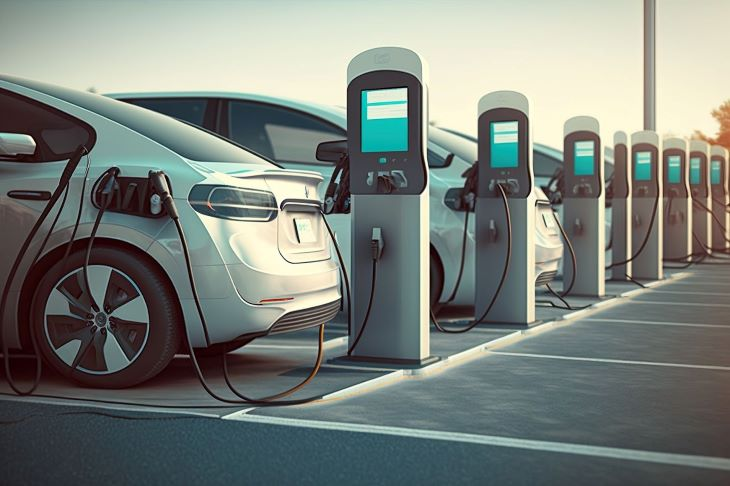
\includegraphics[scale=0.7]{commercial-ev-charging-station.jpg}

  \large Image Source: \url{https://doppleronline.ca/huntsville/ontario-expands-electric-vehicle-charging-stations/}
  \newline \newline
  \normalsize \textbf{Electric vehicles} (or '\textbf{EVs}') have seen massive growth in popularity in recent years. With more
  traditional car manufacturers entering and innovating in the market, consumers have more options at more affordable
  prices than ever before. This project aims to look at publically released EV models comparing their energy efficiency
  and battery capacity. The automobile market has been in a rough area for consumers with reasonable prices being few
  and far between in both the new, and used markets. On top of that, vehicle owners also have to worry about the cost
  of maintenance and gas. Many may be considering EVs for cheaper fuel, maintenance, or longevity. That being said, EVs
  come with their own set of drawbacks, notably the time it takes to charge, and time spent on the road before needing
  to recharge. Of course, purchasing older used models with now inferior technology should yield reduced performance. I
  predict a sharp incline in range from a full charge with more minor improvements being made to fuel efficiency. With
  that being said, are more recent improvements truly substantial enough to overlook the used market entirely? I will be
  taking a thorough look at the relationship between qualitative observations (release year, car type) and quantitative
  observations (battery capacity, energy efficiency, and recharge time). This should give you a good idea of how old is
  too old for EVs, the benefits of buying new as opposed to old EVs, and what you could possibly expect in the years to come.
  \newpage
  \Large Data Collection
  \newline \newline
  \normalsize Natural Resources Canada tracks fuel consumption ratings of vehicles sold in Canada from 1995 to the present
  day. A subset of this data limited to EVs is available on the Open Canada Data website. Due to personal concerns regarding
  the permanence of the csv in it's current state, the data is loaded locally from a file rather than directly from the website.
  \newline \newline
  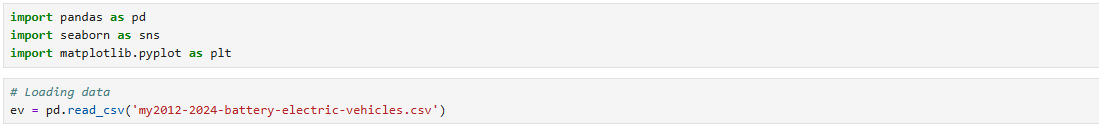
\includegraphics[width=\textwidth]{code_01.png}
  \newline \newline
  \Large Data Cleaning
  \newline \newline
  \normalsize For the purposes I intended to use the dataset for, it was a complete mess. I started by removing columns I
  deemed were unnecessary, many being values regarding CO2 which yields the same result in every vehicle since electric cars
  don't emit CO2. Other removed columns measured how much energy was used in terms of litres of gas. While this is an
  interesting statistic it is irrelevant to the questions I answer through the analysis. While removing these columns aren't
  required, it makes the rest of the cleanup a lot easier. Next was renaming some columns with strange or awkward labels,
  this was also done for many entries in the "Vehicle Class" column.
  \newline \newline
  Finally, Vehicle Classes according to the dataset is split into 16 categories, many of which are only utilized a few times.
  Since weight can have a significant impact on fuel efficiency, cars were assigned a "Weight Class" in a new column based on
  their "Vehicle Class".
  \newline \newline
  \textbf{Weight Classes were divided into small, medium, and large based on the respective vehicle classes weight description
  from the Natural Resources Canada website [5].}
  \newline \newline
  The head and tail of the dataset after the cleanup is displayed below for anybody that is curious to see the final result.
  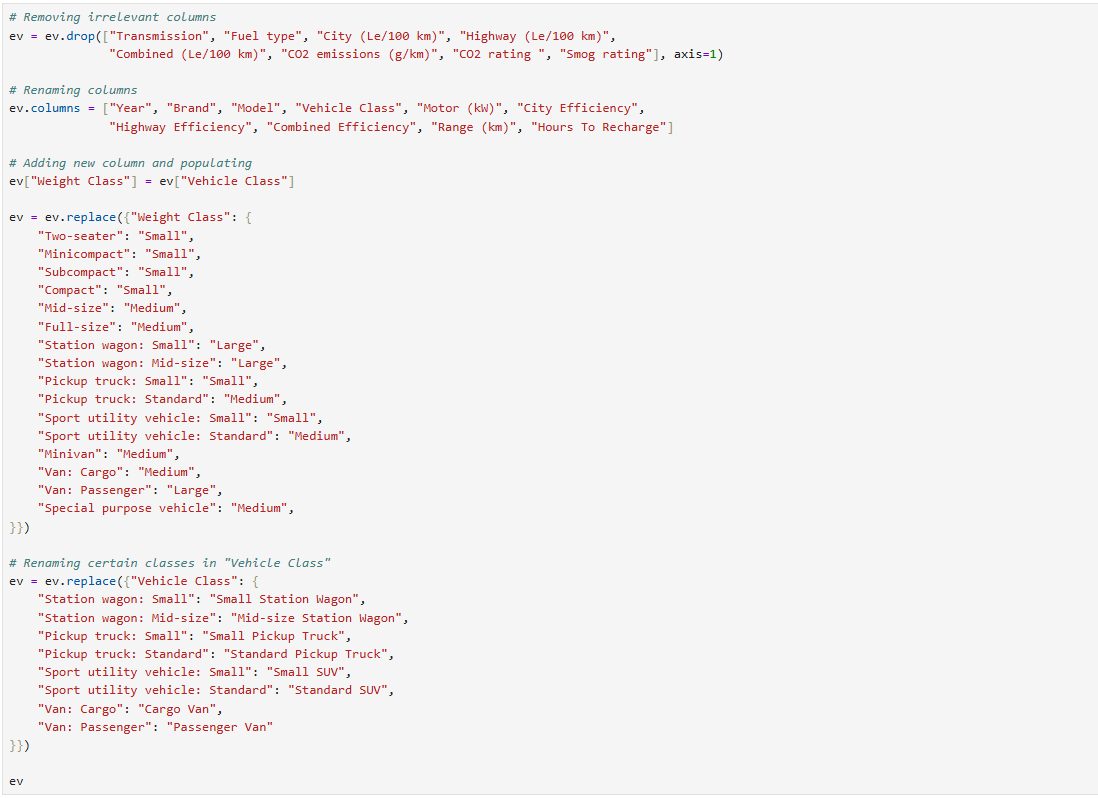
\includegraphics[width=\textwidth]{code_02.png}
  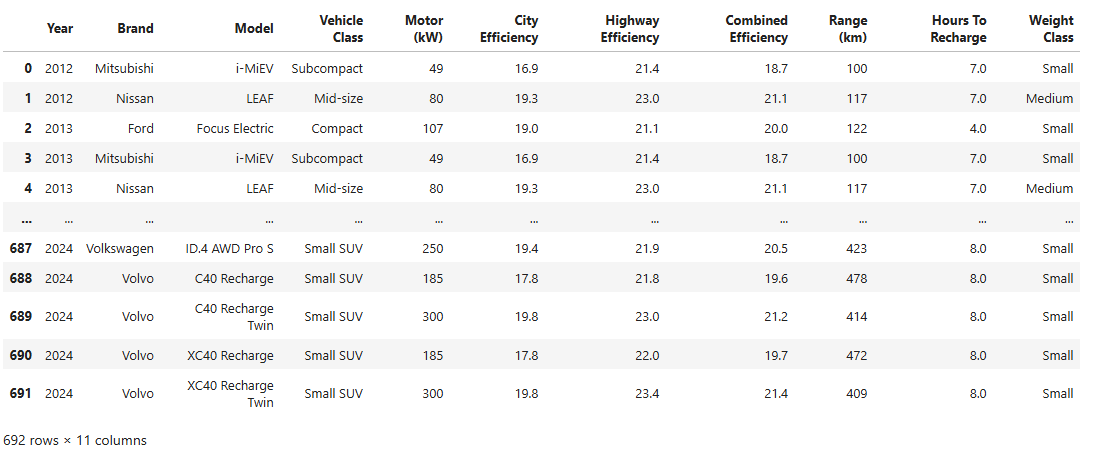
\includegraphics[width=\textwidth]{table_01.png}
  \newpage
  \Large Analysis
  \newline \newline
  \large Distributions
  \newline \newline
  \normalsize Looking at distributions of EVs released throughout the years properly illustrates not only the rapid growth
  in the industry this decade, but also highlights severly low numbers from 2012 - 2015.
  \newline \newline
  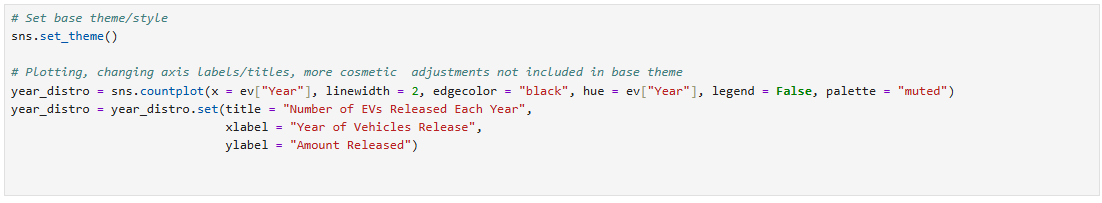
\includegraphics[width=\textwidth]{code_03.png}
  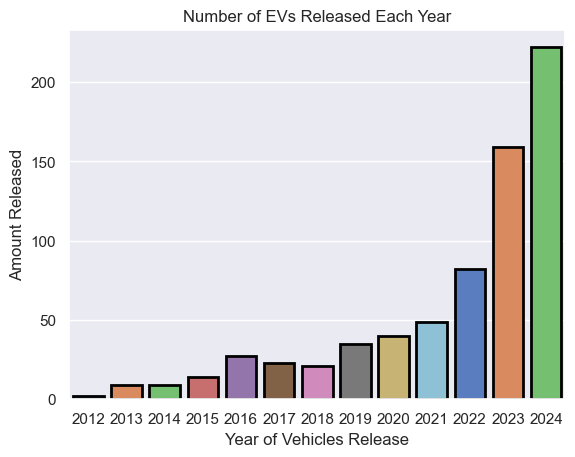
\includegraphics[width=\textwidth]{graph_01.png}
  \newpage
  Checking distributions among the Weight Classes shows a similar lack of data on large EVs.
  \newline \newline
  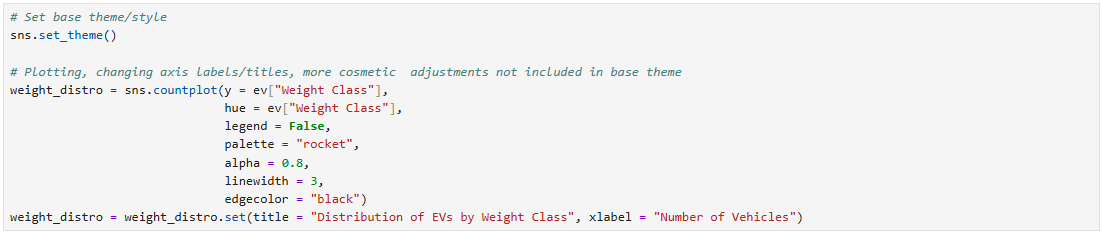
\includegraphics[width=\textwidth]{code_04.png}
  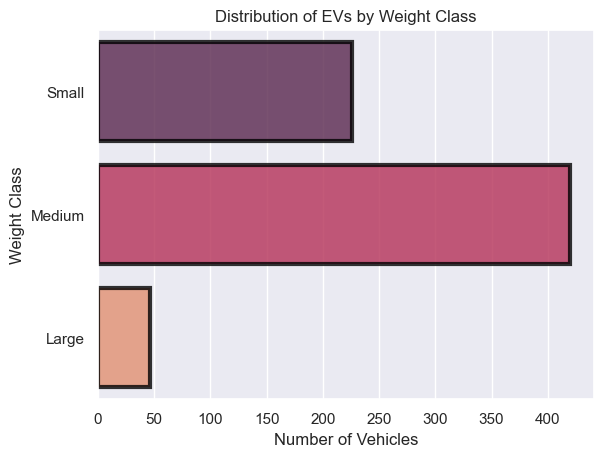
\includegraphics[width=\textwidth]{graph_02.png}
  How may these distributions affect the accuracy of upcoming plots? Graphs using release year in the x axis may contain more
  volatile results in earlier years. As for graphs involving weight class, you'll soon see that data for large vehicles are
  not only more sporadic than it's counterparts, but also lacks any data whatsoever preceding 2015. The table below shows
  weight class distributions per year. Note that prior to 2020 there are at most just 3 large vehicles released per year. While
  this is less than ideal, it further reinforces the importance of dividing the vehicles into weight classes. Had vehicles been
  split by their vehicle class these problems would be amplified to the point where no conclusions could be easily made.
  \newpage
  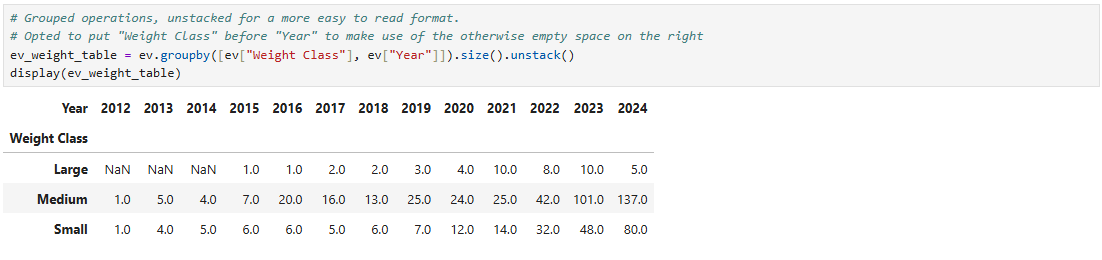
\includegraphics[width=\textwidth]{table_02.png}
  \newline \newline
  \large Improvement (and deterioration) over the years
  \newline \newline
  \normalsize Comparing vehicle range overtime shows steady improvement as the years progress, with a large increase to medium
  vehicles in 2013, and large increases to other vehicles from 2016 - 2020. While improvement almost appears to have plateaued
  recently, there appear to be significant drops in range just 5 years prior to 2024. It is also worth noting that the plateau
  could be a result of the influx of new inexperienced EV manufacturers in recent years.
  \newline \newline
  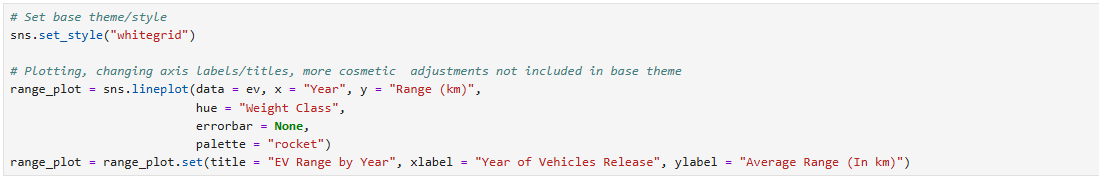
\includegraphics[width=\textwidth]{code_05.png}
  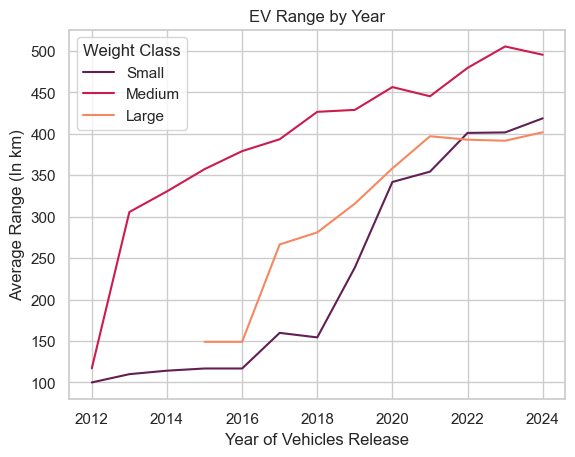
\includegraphics{graph_03.png}
  \newpage
  What I was surprised to discover is that fuel efficiency has actually gotten \textbf{worse} as time progressed. Furthermore,
  after 2017 and until this year large vehicles have been the \textbf{most} fuel efficient.
  \newline \newline
  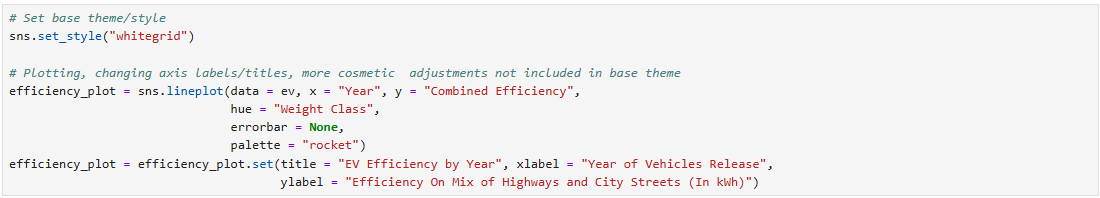
\includegraphics[width=\textwidth]{code_06.png}
  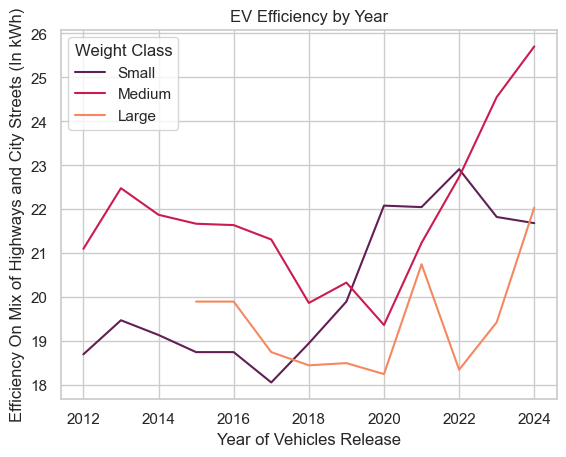
\includegraphics[width=\textwidth]{graph_04.png}
  \newpage
  These results absolutely baffled me at first. How can improved technology result in deterioration of fuel efficiency?
  Well, looking at motors shows that more vehicles in recent years are being made with more powerful motors. This means that
  the vehicle can accelerate more quickly or match acceleration rates compared to lighter vehicles. It appears that EV
  manufacturers were simply not focused on improving fuel efficiency these past years. Additionaly, this push in motor power
  appears to be heavily skewed towards medium vehicles. This provides an adequate explanation for why large vehicles appear to
  be more fuel efficient.
  \newline \newline
  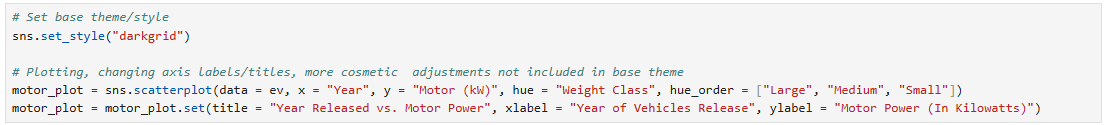
\includegraphics[width=\textwidth]{code_07.png}
  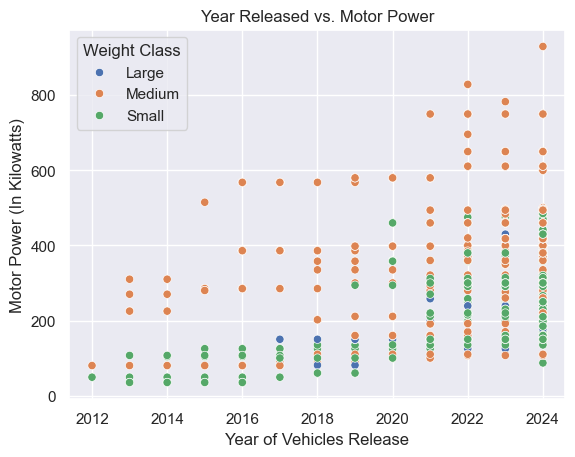
\includegraphics[width=\textwidth]{graph_05.png}
  \newpage
  Finally, charge time has on average increased over the years at a rather unstable rate.
  \newline \newline
  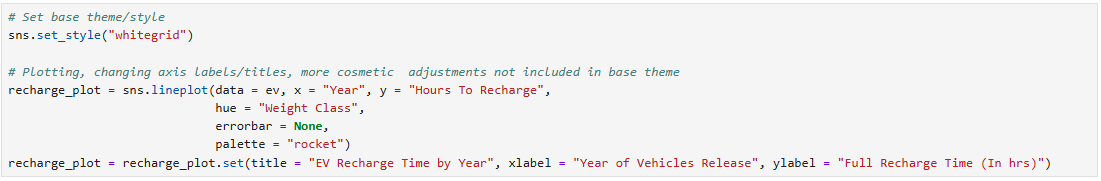
\includegraphics[width=\textwidth]{code_08.png}
  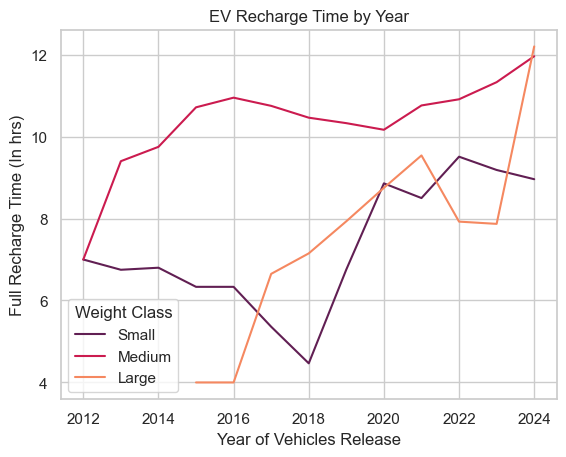
\includegraphics[width=\textwidth]{graph_06.png}
  \newpage
  While not a particularily clean fit, there appears to be a meaningful correlation between recharge time and range. While both
  these values tend to increase with more recent improved technologies, at the moment recharge time appears to be influenced by
  range more than it's year of release.
  \newline \newline
  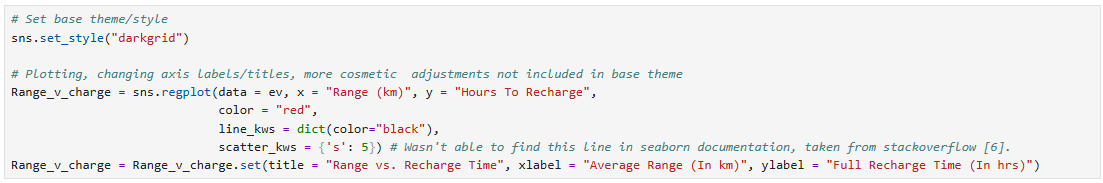
\includegraphics[width=\textwidth]{code_09.png}
  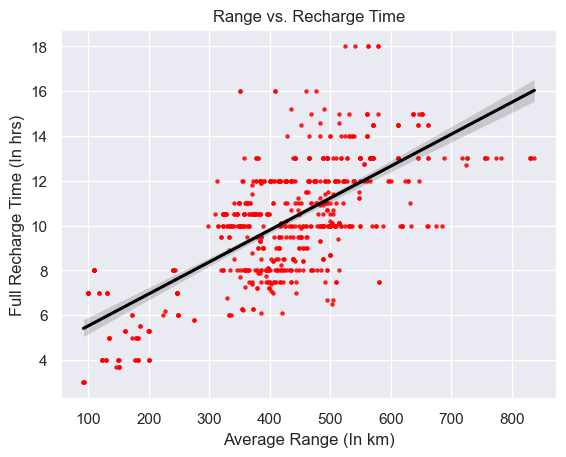
\includegraphics[width=\textwidth]{graph_07.png}
  \newpage
  \Large Discussion
  \newline \newline
  \normalsize Observations from the analysis focused primarily on drawing comparisons between EV performance and a respective
  vehicles year of release. Observations confirmed a substantial increase in average driving range as hypothesized, the most
  egrigous example being an approximate 4x increase over small vehicles. Fuel efficiency however saw it's peak back in the earlier
  days of EVs, with noticibly more electricity being used to power present day vehicles. This contradicts what was hypothesized
  regarding fuel efficiency. This was attributed a trend of increased power in motors, which is shown to have had much higher
  priority to manufacturer's than fuel efficiency to date. While recharge time also trends to higher lengths over the years their
  relationship seems rather volatile. Rather, recharge time appears to be most heavily influenced by vehicle range. But how does
  range increase when fuel efficiency declines? The only other factor that could directly influence range is battery capacity,
  which is unfortunately not included in the dataset. Nevertheless, it is safe to assume using common sense that battery capacity
  is what drives the increase in range. And since a larger battery capacity means more electricity is needed to charge the battery,
  we can conclude that battery size is influencing recharge time.
  \newline \newline
  So how old is too old for a used EV? Well, while a reduced charge time in older models may sound appealing, the reduced range can
  make travelling long distances much more of a hassle. New smaller vehicles have good efficiency although some may need additional
  seating or space to take things on the road with them. Ironically, entering the used market you'll generally have better luck
  with fuel efficiency searching for large vehicles. Given the balance between vehicle range and recharge time I'd recommend trying
  to find used cars from 2020-2023. New cars released in 2024 shouldn't be overlooked either as they yield similar results compared
  to those released after 2020. While the ideal EV will vary depending on individual wants and needs, you should have a much better
  idea of where you should be looking and what to avoid.
  \newline \newline
  \Large References
  \newline \newline \normalsize
  1. Source  Data (published by Natural Resources Canada): \url{https://open.canada.ca/data/en/dataset/98f1a129-f628-4ce4-b24d-6f16bf24dd64/resource/026e45b4-eb63-451f-b34f-d9308ea3a3d9} \newline
  2. Pandas for data manipulation \newline
  3. Seaborn for data vizualization \newline
  4. Matplotlib for data vizualization \newline
  5. "Understanding the tables" from Natural Resources Canada: \url{https://natural-resources.canada.ca/energy-efficiency/transportation-alternative-fuels/personal-vehicles/choosing-right-vehicle/buying-electric-vehicle/understanding-the-tables/21383} \newline
  6. Stackoverflow post from "Max Ghenis" for single line that alters regplot dot size: \url{https://stackoverflow.com/questions/36921550/how-to-change-the-point-size-for-regplot-seaborns-scatter-plot-function-pyt}
}
\end{document}

